\section{Méthodes d'évaluation}

Nous utiliserons le langage de programmation Python pour les deux méthodes.

\subsection{Régression par k plus proches voisins}

L'algorithme des K plus proches voisins (KNN) est un algorithme qui compare directement l'élément test à
une base d'éléments connus sans apprentissage préalable. Cela en fait une solution moins rapide qu'un réseau
de neurones car il nécessite de parcourir les éléments connus à chaque test.\\

Pour chaque vin de notre base, on calcule la distance moyenne quadratique de ses attributs avec le vin à tester.
On garde ensuite les K voisins avec les distances les plus faibles. Dans nôtre cas, on sépare la base en deux sous-bases
distinctes:

\vspace{0.5cm}

\begin{itemize}
    \item Une base d'éléments connus à utiliser pour appliquer l'algorithme.
    \item Une base d'éléments test pour mesurer l'efficacité de l'algorithme.
\end{itemize}

\vspace{0.5cm}

Pour un nombre K de voisins allant de 1 à 20, on mesure:
\vspace{0.5cm}

\begin{itemize}
    \item L'erreur moyenne, 0.6 équivalant à un décalage moyen de 0.6 de qualité prédite avec la qualité connue.
    \item L'accuracy, correspondant au pourcentage de tests dont la qualité prédite correspond à la qualité connue.
\end{itemize}

\vspace{0.5cm}

\begin{figure}[!htb]

    \begin{minipage}{0.5\textwidth}
        \centering
        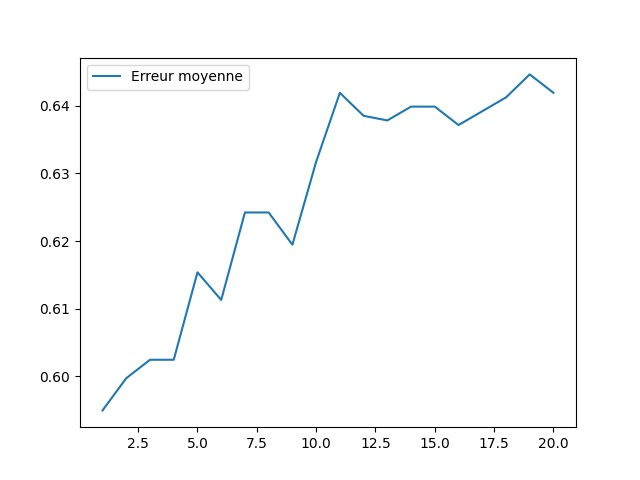
\includegraphics[width=01\textwidth]{../images/knn1.jpeg}
        \label{fig:knn}
    \end{minipage}\hfill

    \begin{minipage}{0.5\textwidth}
        \centering
        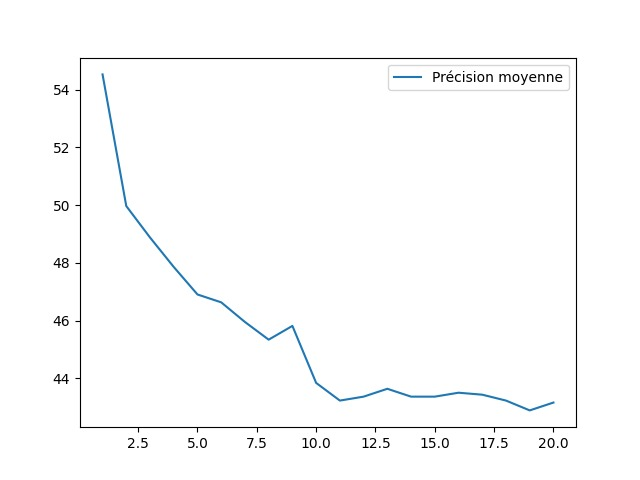
\includegraphics[width=01\textwidth]{../images/knn2.jpeg}
        \label{fig:knn2}
    \end{minipage}\hfill

    \caption{Résultats de l'algorithme KNN}

\end{figure}

\newpage

On peut voir que l'accuracy pour 1 voisin est de 54.5\% et cette dernière diminue si on augmente le nombre de voisins.
Cela parait peut efficace car l'algorithme n'a raison qu'un peu plus d'une fois sur deux. Cependant, il s'agit d'un problème
de régression.

Que l'algorithme se trompe, c'est une chose, mais est-il éloigné de la vérité pour autant? On peut voir que
l'erreur moyenne pour 1 voisin est de moins de 0.6. La qualité d'un vin sera donc notéé en moyenne 0.6 en dessous ou au dessus
de ce qui est attendu, ce qui est peu. Comme pour l'accuracy, on observe qu'avec l'augmentation du nombre de voisins on obtient
de moins bons résultats, l'erreur étant de plus en plus grande.

\vspace{0.5cm}


Cette solution, en restant sur 1 voisin seulement, reste donc une option plutôt satisfaisante.